% Intervention triptych: three variations on the Evolution box from the system
% overview figure, each showing how one knob alters the VLM-selection step of the
% inner evolutionary loop (selection -> mutation/crossover -> offspring grid, x20).
%   Panel A -- Noise   : the x20 loop feeds an epsilon gate that, per draw, routes
%                        to the VLM pick (1-eps) or a random pick (eps)
%                                                (config: rand_select_prob)
%   Panel B -- Memory  : the VLM selects with the last CL grids+picks still behind
%                        the current one in its chat history
%                                                (config: chat_history_turns)
%   Panel C -- Agents  : one persona is sampled (x1, at session start) from a pool
%                        and prepended to the VLM system prompt
%                                                (config: n_personality_traits)
% Self-contained (no external image assets); the generation grid is drawn
% schematically with the selected cell tinted blue to match the VLM-selection node.
% Compile: pdflatex intervention_triptych.tex
%          pdftocairo -svg intervention_triptych.pdf intervention_triptych.svg
\documentclass[border=8pt, varwidth=false]{standalone}
% Shared TikZ styling for the intervention-triptych figure, matching the look of
% paper/system_fig/system_overview.tex and paper/metric_figs. \input after
% \documentclass{standalone}.
\usepackage{tikz}
\usetikzlibrary{positioning,shapes.geometric,arrows.meta,calc,fit,backgrounds,fadings,decorations.pathreplacing}
\usepackage{graphicx}
\usepackage{amsmath,amssymb}
\usepackage{xcolor}
\usepackage[T1]{fontenc}

\tikzset{
  >=Stealth,
  box/.style       = {draw, rounded corners=2pt, align=center,
                      inner sep=4pt, line width=0.6pt, fill=white},
  vlmbox/.style    = {box, fill=blue!5,   draw=blue!55!black},
  mutbox/.style    = {box, fill=green!6,  draw=green!55!black},
  databox/.style   = {box, fill=black!3,  draw=black!45},
  % persona pool/sample tinted orange to match the swept-knob badge (the number of
  % personalities is the thing the Agents sweep varies), echoing Noise's orange gate
  perscard/.style  = {box, fill=orange!12, draw=orange!75!black, align=left},
  img/.style       = {draw=black!45, line width=0.4pt, inner sep=0, outer sep=0},
  cell/.style      = {draw=black!45, line width=0.35pt, fill=black!8,
                      minimum size=0.6cm, inner sep=0},
  % the selected candidate is tinted to match the (blue) VLM-selection node
  selcell/.style   = {cell, draw=blue!55!black, line width=1.1pt, fill=blue!12},
  % faded grid + selection, used for the "past turns" stacked behind in Memory;
  % faint orange tint ties the stacked turns (whose COUNT is the swept CL knob) to
  % the orange sweep badge, matching Noise's orange gate
  ghostcell/.style = {draw=orange!40, line width=0.3pt, fill=orange!6,
                      minimum size=0.6cm, inner sep=0},
  ghostsel/.style  = {ghostcell, draw=blue!35, line width=0.7pt, fill=blue!7},
  pipe/.style      = {->, line width=0.7pt, draw=black!75},
  loop/.style      = {->, line width=0.7pt, draw=blue!55!black, dashed},
  feed/.style      = {->, line width=0.9pt, draw=orange!75!black},
  memfeed/.style   = {->, line width=0.9pt, draw=violet!55!black},
  frame/.style     = {draw=black!45, line width=0.5pt, rounded corners=4pt,
                      inner sep=10pt},
  colTitle/.style  = {font=\bfseries, anchor=south west},
  subTitle/.style  = {font=\scriptsize\itshape, anchor=north west, text=black},
  knob/.style      = {box, fill=orange!12, draw=orange!75!black, line width=0.8pt,
                      font=\scriptsize, anchor=south},
}


% ---- shared geometry ----
\def\PW{8.2}        % panel (frame) width  (cm, x=1cm)
\def\PH{7.3}        % panel (frame) height
\def\selY{-1.8}     % VLM-selection node y (Memory/Agents spine)
\def\mutY{-3.5}     % Mutation/crossover node y
\def\gridY{-5.6}    % generation-grid centre y (aligned across all three panels)
% per-panel frame widths and content centres (x).  Panels are NOT equal width:
% Memory is narrow (little side content), Agents is wide (pool + persona texts).
\def\WA{7.0}\def\WB{6.4}\def\WC{10.2}   % frame widths: Noise / Memory / Agents
\def\GAP{0.5}                           % gap between frames

% draw a 3x2 candidate grid centred at (#1,#2); the cell at (col #3,row #4) is
% highlighted.  #5 = base cell style, #6 = highlighted cell style.
\newcommand{\gridcells}[6]{%
  \foreach \gc in {0,1,2}{%
    \foreach \gr in {0,1}{%
      \pgfmathsetmacro\ix{#1+(\gc-1)*0.66}%
      \pgfmathsetmacro\iy{#2+(0.5-\gr)*0.66}%
      \pgfmathtruncatemacro\ishi{(\gc==#3)&&(\gr==#4)?1:0}%
      \ifnum\ishi=1\node[#6] at (\ix,\iy) {};\else\node[#5] at (\ix,\iy) {};\fi
    }%
  }%
}

% common spine (Memory / Agents): VLM selection -> Mutation/crossover ->
% offspring grid, with the x20 back-edge feeding selection.
\newcommand{\spine}[2]{%
  \pgfmathsetmacro\cx{#2}%  #2 = absolute content-centre x
  \node[vlmbox] (#1sel) at (\cx,\selY) {VLM selection};
  \node[mutbox] (#1mut) at (\cx,\mutY) {Mutation/crossover};
  \draw[pipe] (#1sel) -- (#1mut);
  \gridcells{\cx}{\gridY}{1}{0}{cell}{selcell}%
  \node[draw=none, minimum width=2.1cm, minimum height=1.45cm, inner sep=0]
    (#1grid) at (\cx,\gridY) {};
  \draw[pipe] (#1mut) -- (#1grid.north);
  % x20 back-edge: a clean rightward bulge that arrives into VLM selection
  % horizontally (head clearly points left INTO the node).  The schematic grid is
  % nearly as wide as the selection box, so we cannot rely on a final |- segment
  % (it would vanish); the symmetric horizontal control points give the head.
  \draw[loop] (#1grid.east) .. controls +(1.5,0) and +(1.5,0) ..
    node[pos=0.5, right=-1pt, font=\scriptsize\itshape] {$\times 20$} (#1sel.east);
}

% mock-3D die (cabinet projection) with its front face centred at (#1,#2); used
% by the Noise panel, drawn BEFORE the random-pick node so it peeks out behind it.
\newcommand{\dieiso}[2]{%
  \def\dh{0.21}% half front-face side
  \def\dd{0.15}% depth offset (up-right)
  % right face (darkest)
  \fill[black!16, draw=black!55, line width=0.4pt]
    (#1+\dh,#2-\dh) -- (#1+\dh+\dd,#2-\dh+\dd) --
    (#1+\dh+\dd,#2+\dh+\dd) -- (#1+\dh,#2+\dh) -- cycle;
  % top face (medium)
  \fill[black!7, draw=black!55, line width=0.4pt]
    (#1-\dh,#2+\dh) -- (#1-\dh+\dd,#2+\dh+\dd) --
    (#1+\dh+\dd,#2+\dh+\dd) -- (#1+\dh,#2+\dh) -- cycle;
  % front face (white) + its three pips (a "3")
  \fill[white, draw=black!55, line width=0.4pt]
    (#1-\dh,#2-\dh) rectangle (#1+\dh,#2+\dh);
  \foreach \px/\py in {-0.1/0.1, 0/0, 0.1/-0.1}{%
    \fill[black!75] (#1+\px,#2+\py) circle (0.024);}%
  % two pips on the top face
  \foreach \px/\py in {-0.07/-0.04, 0.06/0.05}{%
    \fill[black!45] (#1+\px+0.5*\dd,#2+\dh+0.5*\dd+\py) circle (0.019);}%
}

\begin{document}
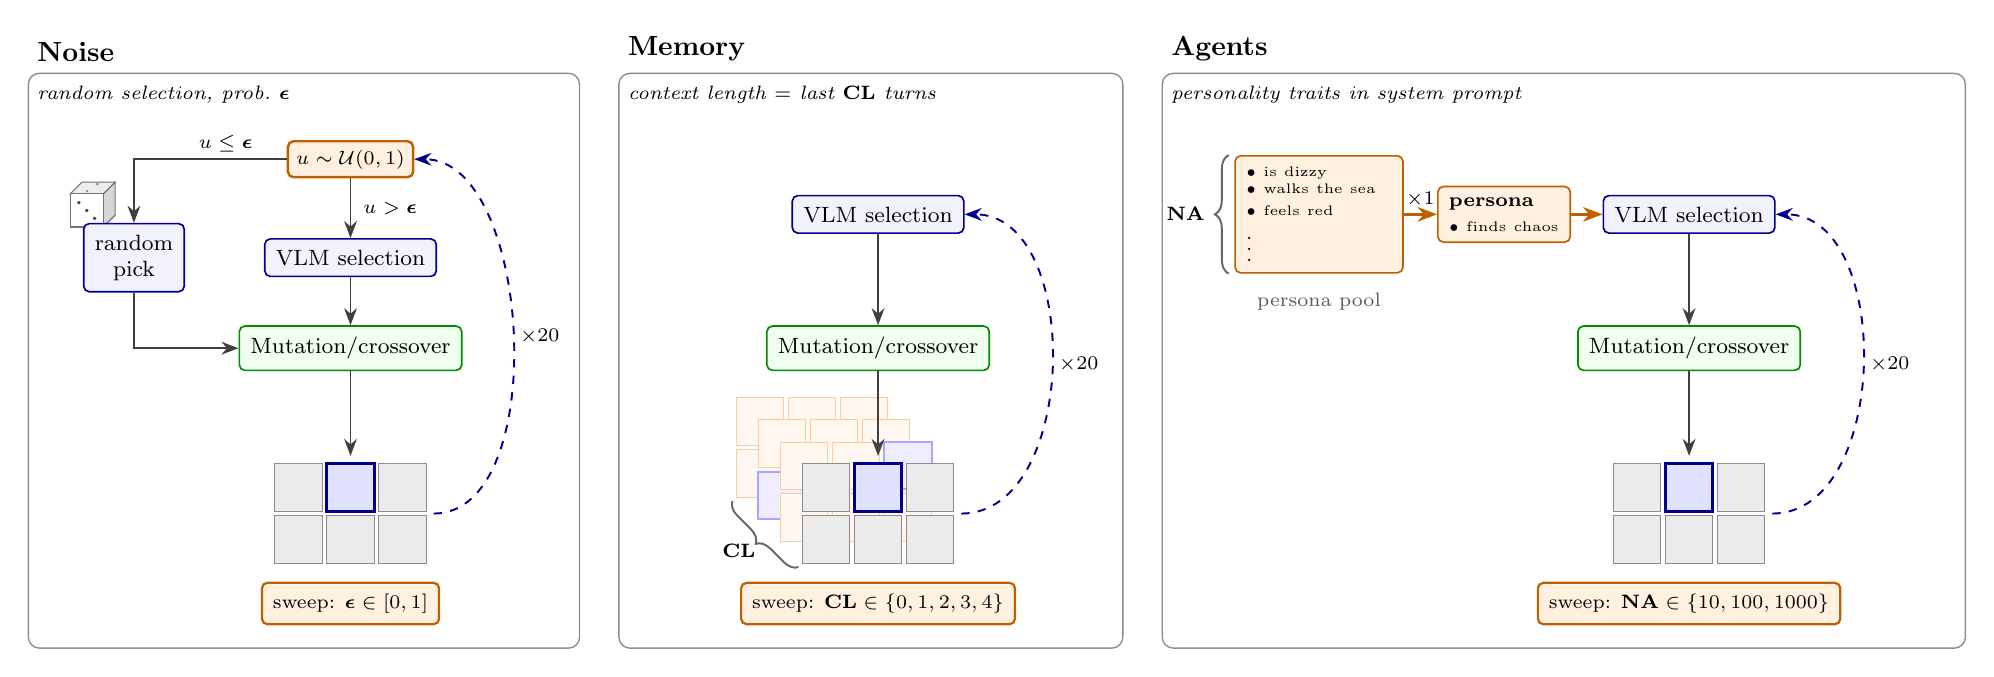
\begin{tikzpicture}[font=\footnotesize, x=1cm, y=1cm]

% panel-left x-origins (each panel its own width; gaps between)
\def\Ax{0}
\pgfmathsetmacro\Bx{\WA+\GAP}
\pgfmathsetmacro\Cx{\WA+\GAP+\WB+\GAP}
% content centres
\pgfmathsetmacro\acx{\Ax+4.1}   % Noise (content pulled left, less dead margin)
\pgfmathsetmacro\bcx{\Bx+3.3}   % Memory (recentred for the narrower frame)
\pgfmathsetmacro\ccx{\Cx+6.7}   % Agents (room on the left for pool + persona)

% ============================== PANEL FRAMES ==============================
\node[frame, minimum width=\WA cm, minimum height=\PH cm, anchor=north west] at (\Ax,0) {};
\node[frame, minimum width=\WB cm, minimum height=\PH cm, anchor=north west] at (\Bx,0) {};
\node[frame, minimum width=\WC cm, minimum height=\PH cm, anchor=north west] at (\Cx,0) {};

% ============================== A: NOISE ==============================
% Custom spine: an epsilon gate sits ABOVE selection and receives the x20 loop;
% it routes to VLM selection (1-eps) or to a random pick (eps), both of which
% feed Mutation/crossover.  (\acx defined above.)
% the gate draws a uniform random variate u; the outgoing edges are guarded on u
\node[draw=orange!75!black, fill=orange!12, rounded corners=2pt, line width=0.9pt,
      inner sep=3pt, font=\scriptsize] (agate) at (\acx,-1.1) {$u\sim\mathcal{U}(0,1)$};
\node[vlmbox] (asel) at (\acx,-2.35) {VLM selection};
\node[mutbox] (amut) at (\acx,\mutY) {Mutation/crossover};
% mock-3D die drawn first so it peeks out from BEHIND the random-pick node's
% top-left corner (clear of the epsilon arrow, which drops into the box's north).
% Positioned so the front face's bottom-right corner sits where the old flat die's
% did relative to the node (node centre + (-0.39,+0.39)).
\dieiso{\Ax+0.75}{-1.75}
\node[vlmbox, align=center] (arand) at (\Ax+1.35,-2.35) {random\\ pick};
\gridcells{\acx}{\gridY}{1}{0}{cell}{selcell}
\node[draw=none, minimum width=2.1cm, minimum height=1.45cm, inner sep=0]
  (agrid) at (\acx,\gridY) {};
% guarded edges -> the two selection modes (u<=eps -> random, prob eps;
% u>eps -> VLM, prob 1-eps)
\draw[pipe] (agate.south) -- (asel.north)
  node[pos=0.5, right=1pt, font=\scriptsize] {$u>\boldsymbol{\epsilon}$};
\draw[pipe] (agate.west) -| (arand.north)
  node[pos=0.2, above=-1pt, font=\scriptsize] {$u\le\boldsymbol{\epsilon}$};
% both selection modes -> Mutation/crossover
\draw[pipe] (asel.south) -- (amut.north);
\draw[pipe] (arand.south) |- (amut.west);
\draw[pipe] (amut.south) -- (agrid.north);
% x20 loop: offspring grid -> gate (the selection decision); clean rightward
% bulge so the head clearly points left INTO the gate
\draw[loop] (agrid.east) .. controls +(1.5,0) and +(1.5,0) ..
  node[pos=0.5, right=-1pt, font=\scriptsize\itshape] {$\times 20$} (agate.east);
\node[colTitle] at (\Ax,0.02) {Noise};
\node[subTitle] at (\Ax,-0.05) {random selection, prob.\ $\boldsymbol{\epsilon}$};
\node[knob] at (\acx,-\PH+0.28) {sweep: $\boldsymbol{\epsilon} \in [0,1]$};

% ============================== B: MEMORY ==============================
% The chat history is shown as faded copies of the candidate grid -- each a past
% turn with a different pick -- stacked behind the current grid along a depth
% diagonal; a brace over the diagonal is labelled CL (context length).
% (\bcx defined above.)
\gridcells{\bcx-0.84}{\gridY+0.84}{2}{1}{ghostcell}{ghostsel}%  oldest turn (back)
\gridcells{\bcx-0.56}{\gridY+0.56}{0}{1}{ghostcell}{ghostsel}%
\gridcells{\bcx-0.28}{\gridY+0.28}{2}{0}{ghostcell}{ghostsel}%  previous turn
\spine{b}{\bcx}
% brace along the depth diagonal (front grid SW -> back grid SW, the bottom-left
% edge of the stack), bulging outward (down-left), labelled CL
\pgfmathsetmacro\bfx{\bcx-0.96}\pgfmathsetmacro\bfy{\gridY-0.63}
\pgfmathsetmacro\bbx{\bcx-1.80}\pgfmathsetmacro\bby{\gridY+0.21}
\draw[decorate, decoration={brace, amplitude=5pt, raise=2pt}, line width=0.7pt,
      draw=black!60]
  (\bfx,\bfy) -- (\bbx,\bby)
  node[midway, below left=2pt, font=\scriptsize] {$\mathbf{CL}$};
\node[colTitle] at (\Bx,0.02) {Memory};
\node[subTitle] at (\Bx,-0.05) {context length $=$ last $\mathbf{CL}$ turns};
\node[knob] at (\bcx,-\PH+0.28) {sweep: $\mathbf{CL} \in \{0,1,2,3,4\}$};

% ============================== C: AGENTS ==============================
% One persona is sampled (x1, once at session start) from a broad pool of
% personalities and prepended to the VLM's system prompt.
\spine{c}{\ccx}
\pgfmathsetmacro\cpoolx{\Cx+2.0}
\pgfmathsetmacro\cperx{\Cx+4.35}
% persona pool: the full list of personality traits, with a vertical ellipsis to
% signal the rest of the pool beyond those shown.  Wide enough that each trait
% sits on one line.
\node[perscard, minimum width=2.0cm, text width=1.85cm, align=left, font=\scriptsize]
  (cpool) at (\cpoolx,\selY)
  {\hyphenpenalty=10000\exhyphenpenalty=10000\relax
   {\tiny $\bullet$ is dizzy\\ $\bullet$ walks the sea\\ $\bullet$ feels red}\\[1pt]
   $\vdots$};
\node[font=\scriptsize, anchor=north, align=center, text=black!65]
  at ([yshift=-0.12cm]cpool.south) {persona pool};
% brace down the left of the persona pool: the pool holds NA personalities (the
% swept knob); a single one is then sampled (the x1 feed below)
\draw[decorate, decoration={brace, amplitude=5pt, raise=2pt}, line width=0.7pt,
      draw=black!60]
  (cpool.south west) -- (cpool.north west)
  node[midway, left=7pt, font=\scriptsize] {$\mathbf{NA}$};
% one trait is sampled (x1, once at session start) -> the persona
\node[perscard, minimum width=1.55cm, text width=1.4cm, align=left, font=\scriptsize]
  (cper) at (\cperx,\selY)
  {\textbf{persona}\\[1pt] {\tiny $\bullet$ finds chaos}};
\draw[feed] (cpool.east) -- (cper.west)
  node[midway, above=-1pt, font=\scriptsize\itshape] {$\times 1$};
\draw[feed] (cper.east) -- (csel.west);
\node[colTitle] at (\Cx,0.02) {Agents};
\node[subTitle] at (\Cx,-0.05) {personality traits in system prompt};
\node[knob] at (\ccx,-\PH+0.28) {sweep: $\mathbf{NA} \in \{10,100,1000\}$};

\end{tikzpicture}
\end{document}
